\documentclass[11pt, a4paper]{article}
\usepackage[utf8]{inputenc}
\usepackage[spanish]{babel}
\usepackage{amsmath, amssymb, amsfonts}
\usepackage{graphicx}
\usepackage{geometry}
\geometry{left=2.5cm, right=2.5cm, top=2.5cm, bottom=2.5cm}
\usepackage{tikz}
\usepackage{bm}
\usepackage[hidelinks]{hyperref}
\graphicspath{{figs/}{../figs/}}

% Línea discontinua entre ejercicios
\newcommand{\separador}{\par\vspace{0.3cm}\noindent\begin{tikzpicture}\draw[dashed] (0,0) -- (\linewidth,0);\end{tikzpicture}\par\vspace{0.3cm}}

\title{\vspace{-1.5cm}\textbf{Resolución de Ecuaciones Diferenciales Ordinarias}\\ \large Métodos Matemáticos I --- Hoja 1}
\author{\textbf{César Endris Acosta}}

\date{10 de septiembre de 2026}
\begin{document}

\maketitle
\vspace{-0.2cm}

\begin{center}
\fbox{\parbox{0.93\linewidth}{\small
\textbf{Versión interactiva.} Todos los problemas de esta hoja se pueden visualizar e interactuar con sus gráficas
(constantes con deslizadores, curva elegida, campos de direcciones, etc.) en la página web
(pestaña ``Hoja 1''):\\[2pt]
\centerline{\url{https://endris10.github.io/Mathematical_Methods_1/}}\vspace{2pt}
Se utilizó IA (Claude, de Anthropic) \textbf{únicamente para programar la página web};
la resolución de las ecuaciones diferenciales es propia.}}
\end{center}

\noindent\textbf{1. Integrad la EDO: $\bm{(1+y^2)dx + (1+x^2)dy = 0}$} \\
\begin{align*}
\frac{dx}{1+x^2} &= -\frac{dy}{1+y^2}
\end{align*}
$y = \tan(\theta) \implies dy = \sec^2(\theta)\,d\theta,\ \ 1+y^2=\sec^2(\theta)$.
\[
\int \frac{dy}{1+y^2} = \int \frac{\sec^2(\theta)\,d\theta}{\sec^2(\theta)} = \int d\theta = \theta = \arctan(y)
\]
\begin{align*}
\arctan(x) &= -\arctan(y) + C
\end{align*}
\textit{Los denominadores $1+x^2$ y $1+y^2$ son siempre positivos ($\geq 1$) $\forall x,y\in\mathbb{R}$, por lo que no existe singularidad ni restricción de signo sobre $C$.}
\[
\boxed{\arctan(x) + \arctan(y) = C}
\]



\begin{center}
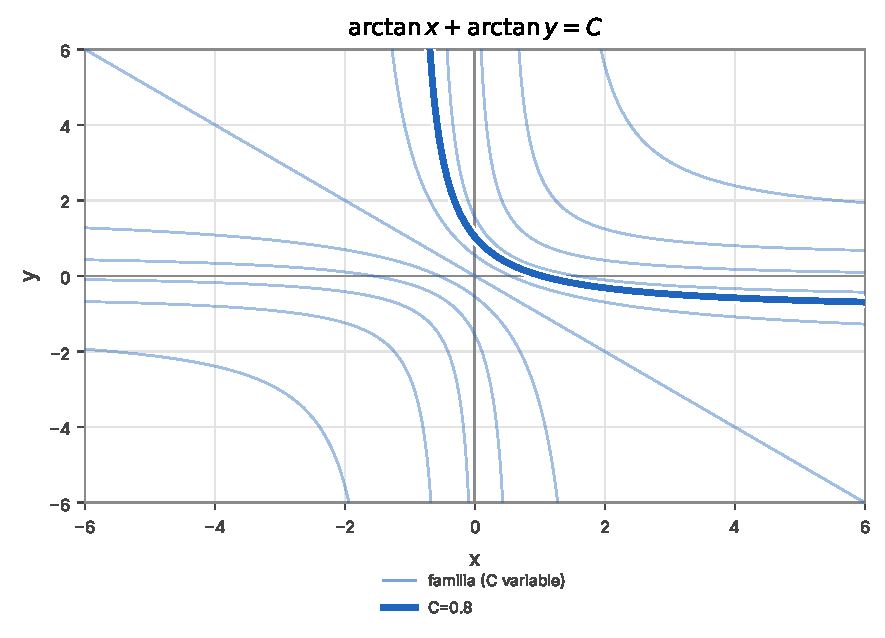
\includegraphics[width=0.8\linewidth]{h1-01.pdf}
\end{center}

\noindent\textbf{2. Integrad la EDO: $\bm{(1+y^2)dx + xydy = 0}$} \\
\begin{align*}
\frac{dx}{x} &= -\frac{y}{1+y^2}dy
\end{align*}
$u = 1+y^2 \implies du = 2y\,dy $.
\[
\int \frac{y}{1+y^2}dy = \int \frac{du/2}{u} = \frac{1}{2}\ln|u| = \frac{1}{2}\ln(1+y^2)
\]
\begin{align*}
\int \frac{dx}{x} &= -\frac{1}{2}\int \frac{du}{u} \\
\ln|x| &= -\frac{1}{2}\ln(1+y^2) + C
\end{align*}
\textit{Al dividir por $x$ se excluye $x=0$; sustituyendo en la ecuación original, $(1+y^2)\cdot 0 + 0\cdot y\,dy=0$ se cumple, así que la recta $x=0$ es también solución. En el caso ($x\neq0$), al despejar $x= \pm Ke^{-\frac12\ln(1+y^2)}$ con $K>0$, pero como $x^2(1+y^2)\geq0$ siempre, la constante final debe cumplir $K\geq0$ (con $K=0$ recuperando la solución singular $x=0$).}
\[
\boxed{x^2(1+y^2) = K, \qquad K\geq 0}
\]



\begin{center}
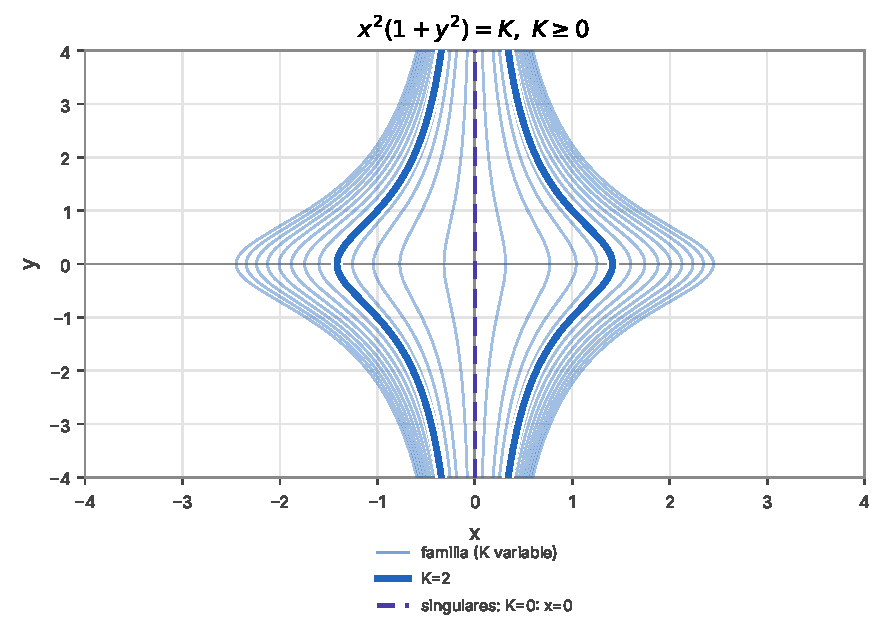
\includegraphics[width=0.8\linewidth]{h1-02.pdf}
\end{center}

\noindent\textbf{3. Integrad la EDO: $\bm{y'\sin(x)-y\cos(x)=0}$ con la condición inicial $\bm{y(\pi/2)=1}$} \\
\begin{align*}
\frac{dy}{y} &= \frac{\cos(x)}{\sin(x)}dx
\end{align*}
\textit{Al dividir por $y$ se excluye $y=0$; pero si $y\equiv 0$, entonces $y'=0$ y la ecuación original $0\cdot\sin(x)-0\cdot\cos(x)=0$ se satisface $\forall x$, luego $y=0$ es también solución. Con $y\neq0$:}
\begin{align*}
\int \frac{dy}{y} &= \int \cot(x)dx \\
\ln|y| &= \ln|\sin(x)| + C
\end{align*}
Al exponenciar, $|y|=e^C|\sin(x)|$, y separando $y>0$ o $y<0$ se obtiene $y=\pm K\sin(x)$ con $K>0$; incluyendo $K=0$ se recupera el caso singular.
Aplicando $y(\pi/2)=1 \implies 1 = K\sin(\pi/2) \implies K = 1$.
\[
\boxed{y = \sin(x)}
\]



\begin{center}
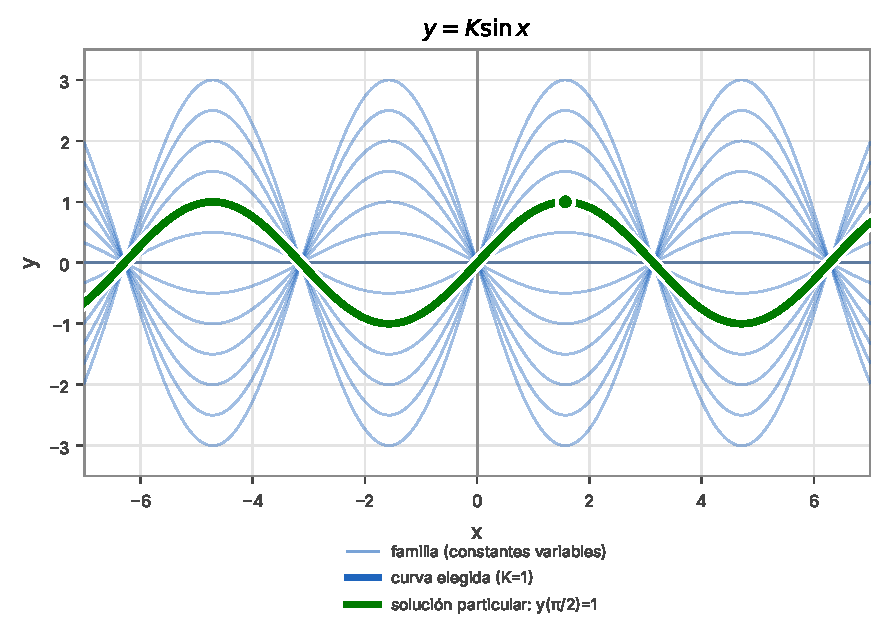
\includegraphics[width=0.8\linewidth]{h1-03.pdf}
\end{center}

\noindent\textbf{4. Integrad la EDO: $\bm{x\sqrt{1+y^2}+yy'\sqrt{1+x^2}=0}$} \\
\begin{align*}
\frac{x}{\sqrt{1+x^2}}dx &= -\frac{y}{\sqrt{1+y^2}}dy
\end{align*}
\[
\int \frac{y}{\sqrt{1+y^2}}dy = \int \frac{du/2}{\sqrt{u}} = \sqrt{u} = \sqrt{1+y^2}
\]
\[
\int \frac{x}{\sqrt{1+x^2}}dx=\sqrt{1+x^2}
\]
\begin{align*}
\sqrt{1+x^2} &= -\sqrt{1+y^2} + C
\end{align*}
\textit{$\sqrt{1+x^2}\geq1$ y $\sqrt{1+y^2}\geq1$ siempre, no hay singularidad, pero sí una restricción: $C\geq2$.}
\[
\boxed{\sqrt{1+x^2} + \sqrt{1+y^2} = C, \qquad C\geq 2}
\]



\begin{center}
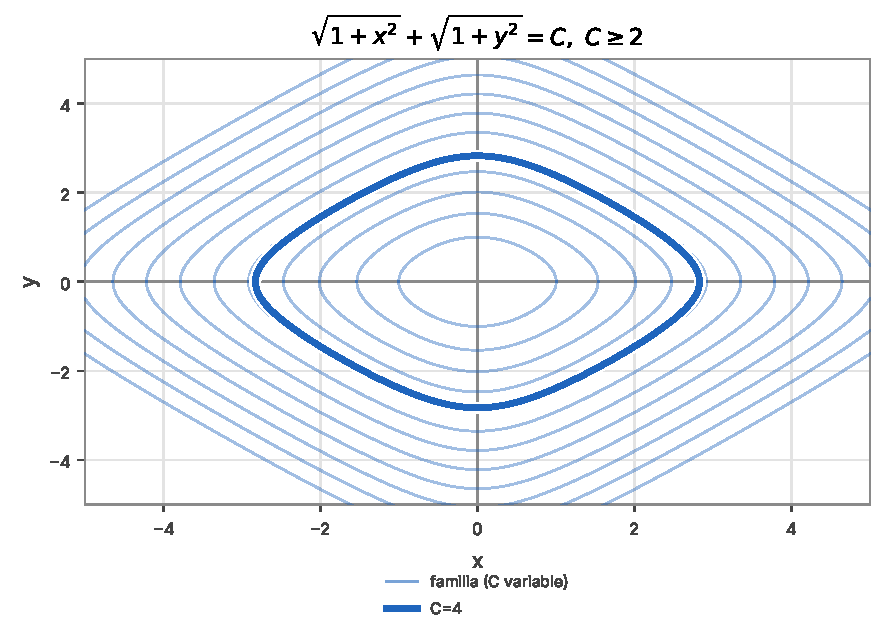
\includegraphics[width=0.8\linewidth]{h1-04.pdf}
\end{center}

\noindent\textbf{5. Integrad la EDO: $\bm{x\sqrt{1-y^2}dx+y\sqrt{1-x^2}dy=0}$ con la condición inicial $\bm{y(0)=1}$} \\
\begin{align*}
\frac{x}{\sqrt{1-x^2}}dx &= -\frac{y}{\sqrt{1-y^2}}dy \\
\int \frac{x}{\sqrt{1-x^2}}dx &= -\int \frac{y}{\sqrt{1-y^2}}dy \\
-\sqrt{1-x^2} &= \sqrt{1-y^2} + C \implies \sqrt{1-x^2} + \sqrt{1-y^2} = K
\end{align*}
\textit{El dominio exige $|x|\leq1$, $|y|\leq1$; en $x=\pm1$ o $y=\pm1$ las raíces se anulan (no constituyen curvas de solución independientes). Como $0\leq\sqrt{1-x^2}\leq1$ y $0\leq\sqrt{1-y^2}\leq1$, se requiere $0\leq K\leq2$.}
Aplicando $y(0)=1 \implies \sqrt{1-0} + \sqrt{1-1} = K \implies K=1$.
\[
\boxed{\sqrt{1-x^2} + \sqrt{1-y^2} = 1}
\]



\begin{center}
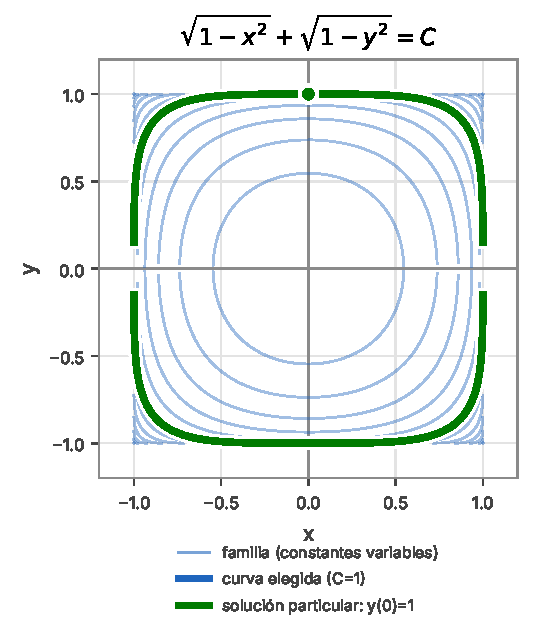
\includegraphics[width=0.8\linewidth]{h1-05.pdf}
\end{center}

\noindent\textbf{6. Integrad la EDO: $\bm{e^{-y}(1+y')=1}$} \\
\begin{align*}
1+y' &= e^y \implies y' = e^y - 1 \implies \frac{dy}{e^y-1} = dx
\end{align*}
\textit{Al dividir por $e^y-1$ se excluye $y=0$; si $y\equiv0$, entonces $y'=0$ y la ecuación original $e^{0}(1+0)=1$ se cumple, luego $y=0$ es también solución (caso singular). En el caso $y\neq0$:}

$u=e^y-1 \implies du=e^y\,dy=(u+1)\,dy \implies dy=\dfrac{du}{u+1}$.
\begin{align*}
\frac{dy}{e^y-1} &= \frac{du/(u+1)}{u} = \frac{du}{u(u+1)} \implies \dfrac{1}{u(u+1)}=( \dfrac{1}{u}-\dfrac{1}{u+1} ){du}.
\end{align*}

\begin{align*}
\int \left(\frac{1}{u}-\frac{1}{u+1}\right)du &= \int dx \\
\ln\left|\frac{u}{u+1}\right| &= x+C
\end{align*}
Deshaciendo el cambio: $\ln\left|\dfrac{e^y-1}{e^y}\right|=x+C \implies \ln|1-e^{-y}|=x+C$.
\textit{Al exponenciar, $K>0$ (sin embargo con $\pm$ se recuperan todas las soluciones, positivo si $y>0$, negativo si $y<0$) y $K=0$ recupera el caso singular $y=0$.}
\[
\boxed{1 - e^{-y} = \pm K e^x}
\]



\begin{center}
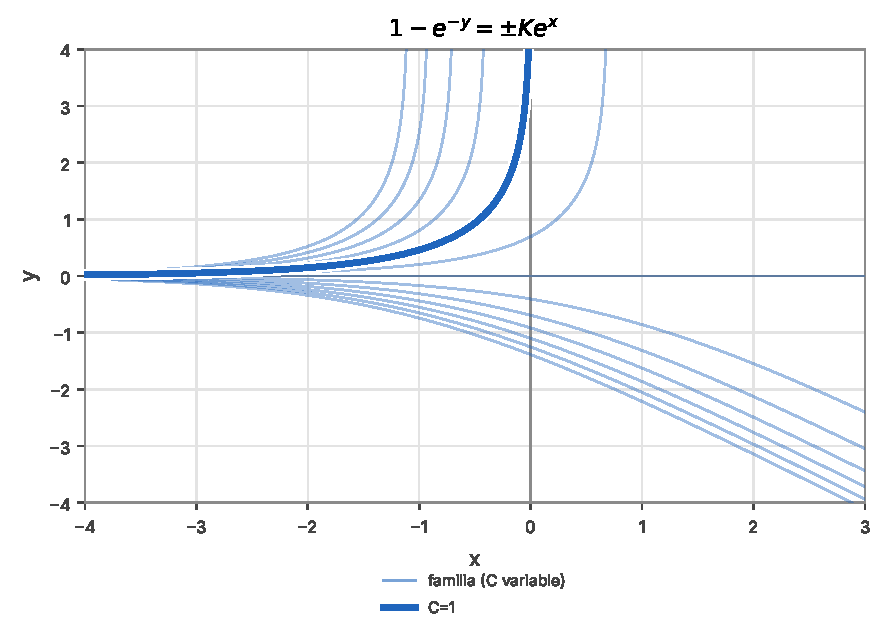
\includegraphics[width=0.8\linewidth]{h1-06.pdf}
\end{center}

\noindent\textbf{7. Integrad la EDO: $\bm{y\ln y \, dx + x \, dy = 0}$ con la condición inicial $\bm{y(1)=1}$} \\
\begin{align*}
\frac{dx}{x} &= -\frac{dy}{y\ln y}
\end{align*}
\textit{El dominio requiere $y>0$; al dividir por $\ln y$ se excluye $y=1$. Si $y\equiv1$, entonces $y'=0$ y la ecuación original $1\cdot\ln(1)\,dx+x\cdot0=0$ se cumple, luego $y=1$ es también solución (caso singular).}

$u = \ln y \implies du = \dfrac{dy}{y}$.
\begin{align*}
\int \frac{dx}{x} &= -\int \frac{du}{u} \\
\ln|x| &= -\ln|u| + C \implies x\ln y = K
\end{align*}
Aplicando $y(1)=1 \implies 1 \cdot \ln(1) = K \implies K = 0$, valor que corresponde al caso hallado arriba.
\[
x\ln y = 0 \implies
\]
\[
\boxed{y = 1}
\]



\begin{center}
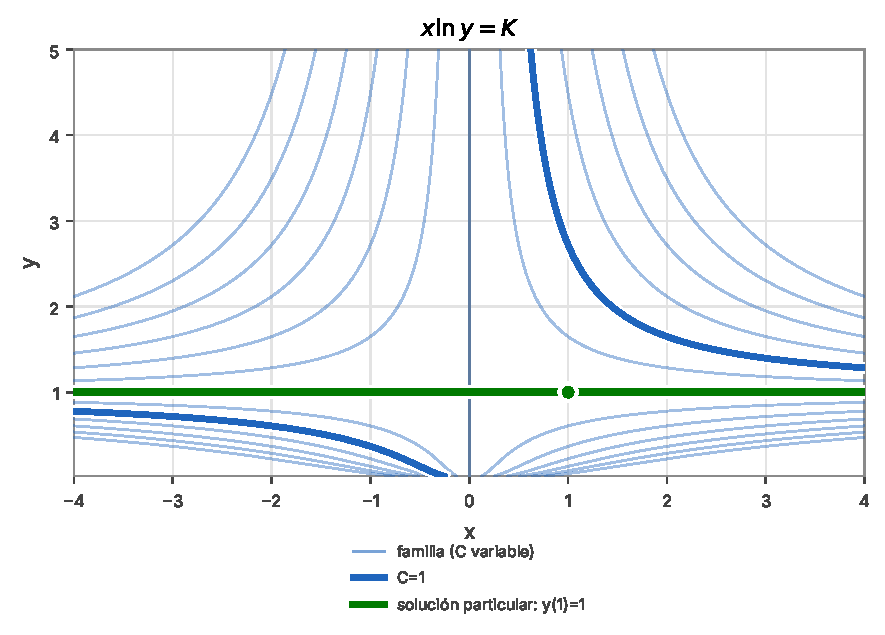
\includegraphics[width=0.8\linewidth]{h1-07.pdf}
\end{center}

\noindent\textbf{8. Integrad la EDO: $\bm{y' = a^{x+y}}$ con $\bm{a>0}$ y $\bm{a \neq 1}$} \\
$z = x+y \implies z' = 1+y' \implies y' = z'-1$.
\begin{align*}
z'-1 &= a^z \implies z' = 1+a^z \implies \frac{dz}{1+a^z} = dx
\end{align*}
$u = 1+a^z \implies du = a^z\ln(a)\,dz = (u-1)\ln(a)\,dz \implies dz = \dfrac{du}{(u-1)\ln a}$.
\[
\frac{dz}{1+a^z} = \frac{dz}{u} = \frac{du}{u(u-1)\ln a} = (\dfrac{1}{u-1}-\dfrac{1}{u})(\frac{du}{\ln a})
\]

\begin{align*}
\int \frac{dz}{1+a^z} &= \frac{1}{\ln a}\int \left(\frac{1}{u-1}-\frac{1}{u}\right)du = \frac{1}{\ln a}\ln\left|\frac{u-1}{u}\right| \\
\frac{1}{\ln a}\ln\left|\frac{u-1}{u}\right| &= x+C
\end{align*}
\textit{Como $a^z>0\ \forall z\in\mathbb{R}$, se tiene $u=1+a^z>1$ siempre, luego $u\neq0$ y $u-1=a^z\neq0$: ningún paso excluye soluciones.}

\[
\ln\left|\frac{a^z}{1+a^z}\right| = x\ln a + C_1 \implies \frac{a^z}{1+a^z} = Ka^x
\]
\begin{align*}
a^z &= Ka^x(1+a^z) \implies a^z(1-Ka^x) = Ka^x \implies a^z = \frac{Ka^x}{1-Ka^x}
\end{align*}

\[
a^xa^y = \frac{Ka^x}{1-Ka^x} \implies a^y = \frac{K}{1-Ka^x} \implies a^{-y} = \frac{1}{K}-a^x
\]
\textit{Como $a^x>0$ y $a^{-y}>0$ para todo $x,y\in\mathbb{R}$ (pues $a>0$), la constante $\dfrac1K$ debe ser positiva: no hay caso de singularidad ni de signo negativo.}
\[
\boxed{a^x + a^{-y} = K, \qquad K>0}
\]



\begin{center}
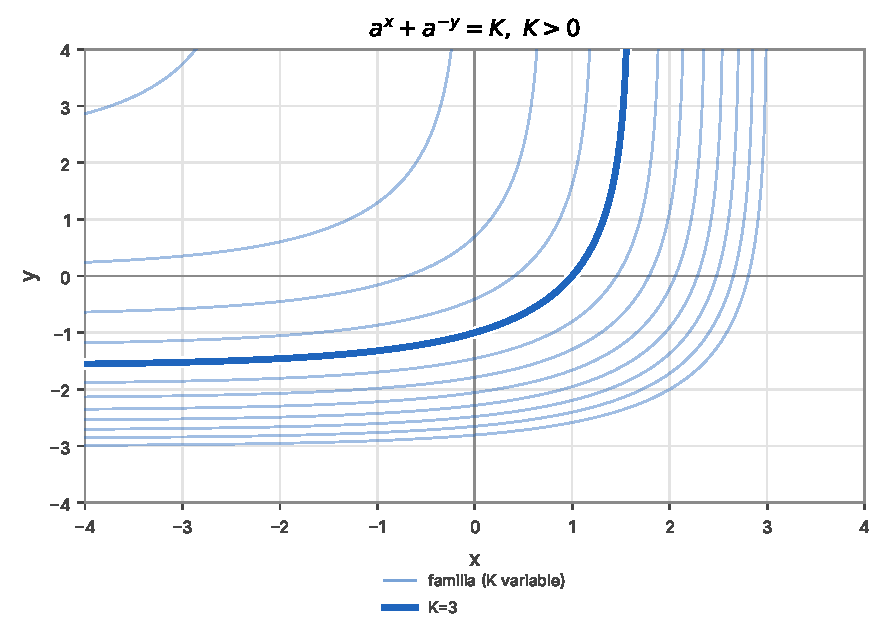
\includegraphics[width=0.8\linewidth]{h1-08.pdf}
\end{center}

\noindent\textbf{9. Integrad la EDO: $\bm{y' = \sin(x-y)}$} \\
$z = x-y \implies z' = 1-y'$.
\[
1-z' = \sin(z) \implies z' = 1-\sin(z) \implies \frac{dz}{1-\sin(z)} = dx
\]

$u=\tan\left(\dfrac{z}{2}\right) \implies du = \dfrac{1+u^2}{2}\,dz \implies dz=\dfrac{2\,du}{1+u^2}$.\quad
\begin{tikzpicture}[baseline={([yshift=-0.6ex]current bounding box.center)}, scale=0.5]
\coordinate (A) at (0,0);
\coordinate (B) at (3,0);
\coordinate (C) at (3,2);
\draw[thick] (A) -- (B) -- (C) -- cycle;
\draw (A) ++(0.35,0) arc (0:33.7:0.35);
\node at (0.62,0.17) {$z$};
\node[below] at (1.5,0) {$1-u^2$};
\node[right] at (3,1) {$2u$};
\node[above, sloped] at (1.15,1) {$1+u^2$};
\draw (2.85,0) -- (2.85,0.15) -- (3,0.15);
\end{tikzpicture}

\begin{align*}
\sin(z) = \frac{2u}{1+u^2} \implies 1-\sin(z) &= \frac{(1-u)^2}{1+u^2} \implies \frac{dz}{1-\sin(z)} = \frac{2\,du}{(1-u)^2} \\
\int \frac{2\,du}{(1-u)^2} &= \int dx \implies \frac{2}{1-u} = x + C
\end{align*}

\textit{Al dividir por $1-\sin(z)$ se excluye $\sin(z)=1$, es decir $z=x-y=\dfrac{\pi}{2}+2k\pi$; sustituyendo, $z'=1-\sin(\pi/2)=0$ concuerda con $z$ constante, luego $y=x-\dfrac{\pi}{2}-2k\pi$ es también solución.}
\[
\boxed{\frac{2}{1-\tan\left(\dfrac{x-y}{2}\right)} = x + C}
\]



\begin{center}
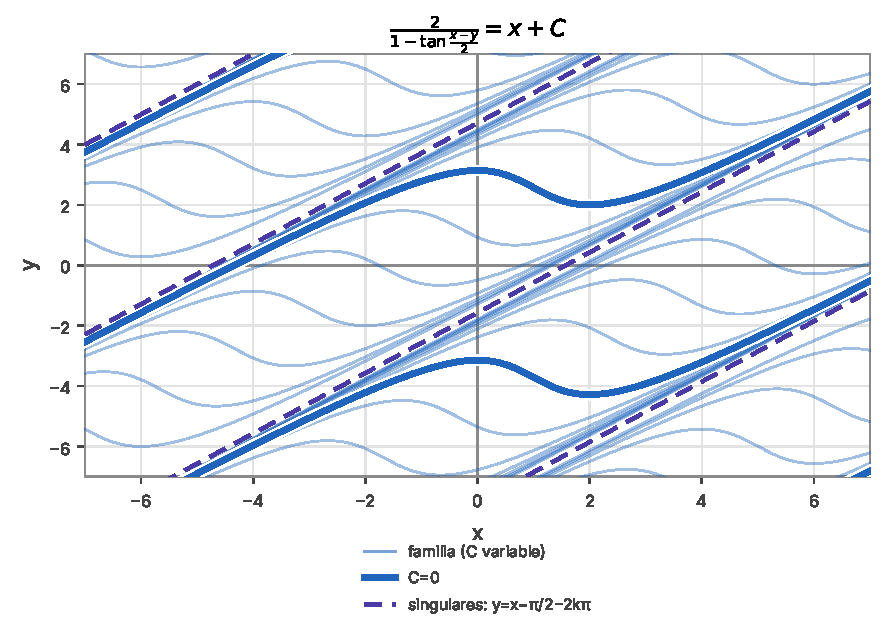
\includegraphics[width=0.8\linewidth]{h1-09.pdf}
\end{center}

\noindent\textbf{10. Integrad la EDO: $\bm{y' = ax+by+c}$ con $\bm{a, b, c}$ constantes} \\
Cambio de variable: $z = ax+by+c \implies z' = a+by' \implies y' = \dfrac{z'-a}{b}$.
\begin{align*}
\frac{z'-a}{b} &= z \implies z' = a+bz \implies \frac{dz}{a+bz} = dx
\end{align*}
\textit{Con $b\neq0$ al dividir por $a+bz$ se excluye $z=-a/b$; en ese punto $z'=a+b(-a/b)=0$, consistente con $z$ constante, luego es también solución.}
\begin{align*}
\int \frac{dz}{a+bz} &= \int dx \\
\frac{1}{b}\ln|a+bz| &= x + C_1 \implies a+bz = \pm K e^{bx}
\end{align*}
Se puede tomar cualquier signo según el signo de $a+bz$ será el elegido en el $\pm$ ; $K=0$ recupera el caso singular.
\[
\boxed{a+b(ax+by+c) = \pm K e^{bx}}
\]



\begin{center}
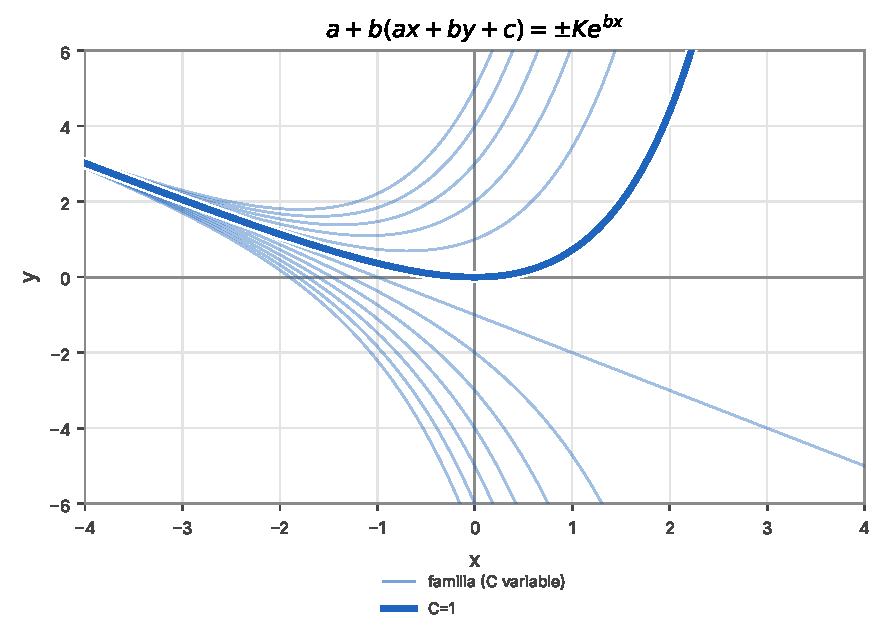
\includegraphics[width=0.8\linewidth]{h1-10.pdf}
\end{center}

\noindent\textbf{11. Integrad la EDO: $\bm{y+xy' = a(1+xy)}$ con la condición inicial $\bm{y(1/a)=-a}$} \\
$z = xy \implies z' = y+xy'$.
\begin{align*}
z' &= a(1+z) \implies \frac{dz}{1+z} = a\,dx
\end{align*}
\textit{Al dividir por $1+z$ se excluye $z=-1$, es decir $xy=-1 \Leftrightarrow y=-1/x$. Comprobación en la ecuación original con $y=-1/x$, $y'=1/x^2$: $y+xy'=-\frac1x+\frac1x=0$ y $a(1+xy)=a(1-1)=0$, luego $y=-1/x$ es también solución, válida para \emph{cualquier} $a$.}
\begin{align*}
\int \frac{dz}{1+z} &= a\int dx \\
\ln|1+z| &= ax + C \implies 1+z = K e^{ax} \implies 1+xy = K e^{ax}
\end{align*}
Aplicando $y(1/a)=-a \implies 1 + \frac{1}{a}(-a) = K e^{a(1/a)} \implies 0 = K e \implies K=0$, valor que coincide con el hallado arriba.
\[
1+xy = 0 \implies
\]
\[
\boxed{y = -\frac{1}{x}}
\]



\begin{center}
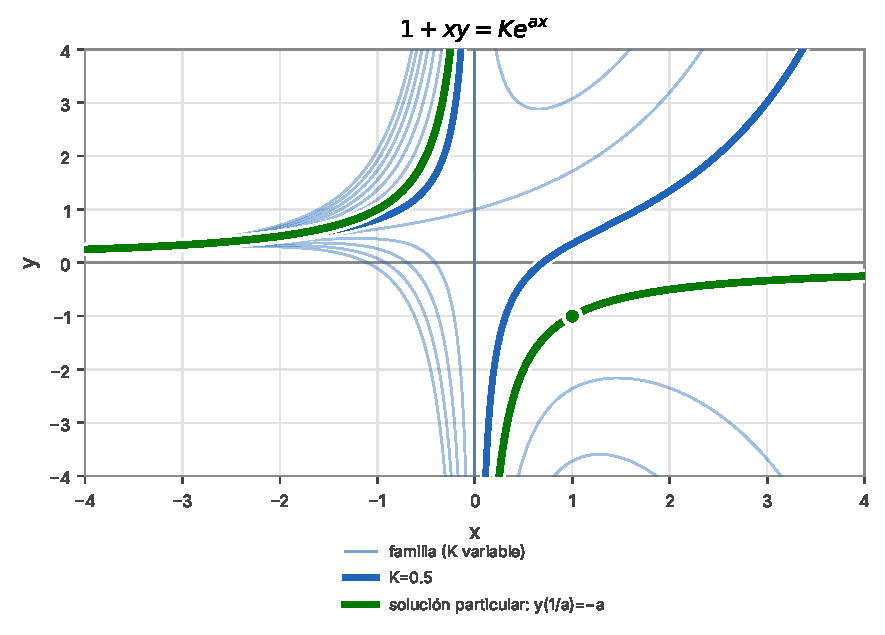
\includegraphics[width=0.8\linewidth]{h1-11.pdf}
\end{center}

\noindent\textbf{12. Integrad la EDO: $\bm{y'+\sin(x-y)=\sin(x+y)}$ con la condición inicial $\bm{y(\pi)=\pi/2}$} \\
Desarrollamos la diferencia de senos paso a paso:
\begin{align*}
\sin(x+y) &= \sin(x)\cos(y) + \cos(x)\sin(y) \\
\sin(x-y) &= \sin(x)\cos(y) - \cos(x)\sin(y)
\end{align*}
\begin{align*}
\sin(x+y) - \sin(x-y) &= \big[\sin(x)\cos(y) + \cos(x)\sin(y)\big] - \big[\sin(x)\cos(y) - \cos(x)\sin(y)\big] \\
&= 2\cos(x)\sin(y)
\end{align*}
Por lo tanto:
\begin{align*}
y' &= 2\cos(x)\sin(y) \implies \frac{dy}{\sin(y)} = 2\cos(x)dx
\end{align*}
\textit{Al dividir por $\sin(y)$ se excluye $y=k\pi$; sustituyendo $y=k\pi$ (constante, $y'=0$) en la ecuación original: $\sin(x-k\pi)=\sin(x+k\pi)=\pm\sin(x)$ (mismo signo en ambos lados), por lo que $0+\sin(x-k\pi)=\sin(x+k\pi)$ se cumple, y $y=k\pi$ es también solución.}

Para integrar $\int \csc(y)\,dy$ : $u=\tan\left(\dfrac{y}{2}\right) \implies dy=\dfrac{2\,du}{1+u^2},\ \sin(y)=\dfrac{2u}{1+u^2}$.
\[
\csc(y)\,dy = \frac{1+u^2}{2u}\cdot\frac{2\,du}{1+u^2} = \frac{du}{u}
\]
\begin{align*}
\int \csc(y)\,dy &= \int \frac{du}{u} = \ln|u| = \ln\left|\tan\left(\frac{y}{2}\right)\right|
\end{align*}
\[
\ln\left|\tan\left(\frac{y}{2}\right)\right| = 2\sin(x) + C
\]
Aplicando $y(\pi)=\pi/2 \implies \ln|\tan(\pi/4)| = 2\sin(\pi)+C \implies \ln(1) = C \implies C=0$.
\[
\boxed{\tan\left(\frac{y}{2}\right) = e^{2\sin(x)}}
\]



\begin{center}
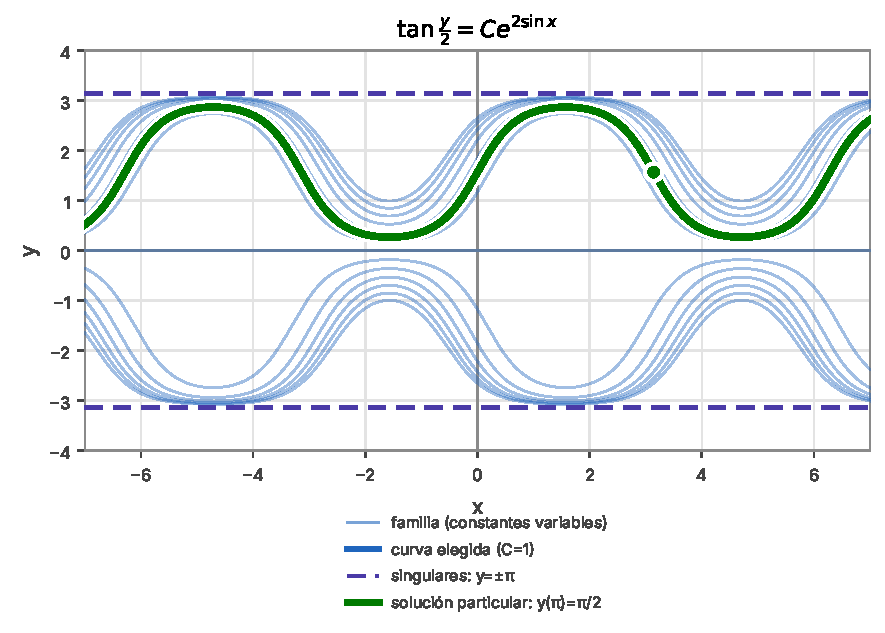
\includegraphics[width=0.8\linewidth]{h1-12.pdf}
\end{center}

\noindent\textbf{13. Integrad la EDO: $\bm{(1+x^2)y' - \frac{1}{2}\cos^2(2y) = 0}$ con $\bm{y \to 7\pi/2}$ cuando $\bm{x \to -\infty}$} \\
\begin{align*}
\frac{2\,dy}{\cos^2(2y)} &= \frac{dx}{1+x^2}
\end{align*}
\textit{Al dividir por $\cos^2(2y)$ se excluye $\cos(2y)=0$, es decir $y=\dfrac{\pi}{4}+\dfrac{k\pi}{2}$; en ese caso $y'=0$ y la ecuación original $(1+x^2)\cdot0-\frac12\cdot0=0$ se cumple, luego esas rectas son también solución.}
\begin{align*}
\int 2\sec^2(2y)\,dy &= \int \frac{dx}{1+x^2} \\
\tan(2y) &= \arctan(x) + C
\end{align*}
Límite $x \to -\infty \implies \arctan(x) \to -\pi/2$ e $y \to 7\pi/2$. \\
$\tan(7\pi) = -\frac{\pi}{2} + C \implies 0 = -\frac{\pi}{2} + C \implies C = \frac{\pi}{2}$.
\[
\boxed{\tan(2y) = \arctan(x) + \frac{\pi}{2}}
\]



\begin{center}
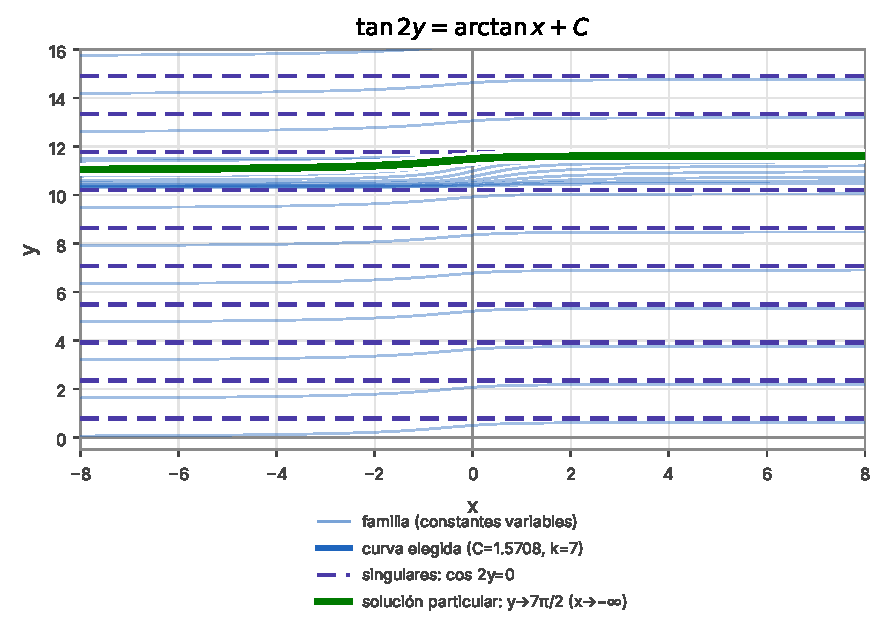
\includegraphics[width=0.8\linewidth]{h1-13.pdf}
\end{center}

\noindent\textbf{14. Integrad la EDO: $\bm{y' = 2x(\pi+y)}$ con $\bm{y}$ acotada cuando $\bm{x \to +\infty}$} \\
\begin{align*}
\frac{dy}{\pi+y} &= 2x\,dx
\end{align*}
\textit{Al dividir por $\pi+y$ se excluye $y=-\pi$; sustituyendo, $y'=0$ y $2x(\pi-\pi)=0$ se cumple para todo $x$, luego $y=-\pi$ es solución.}
\begin{align*}
\int \frac{dy}{\pi+y} &= \int 2x\,dx \\
\ln|\pi+y| &= x^2 + C \implies \pi+y = \pm K e^{x^2} \implies y = \pm K e^{x^2} - \pi
\end{align*}
Para que $y$ esté acotada cuando $x \to +\infty$, $K=0$
\[
\boxed{y = -\pi}
\]



\begin{center}
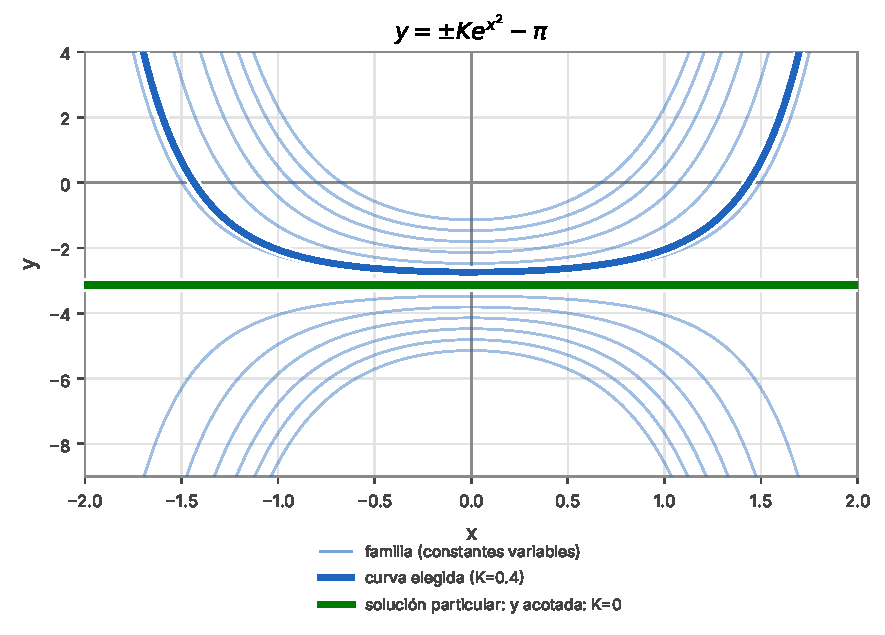
\includegraphics[width=0.8\linewidth]{h1-14.pdf}
\end{center}

\noindent\textbf{15. Integrad la EDO: $\bm{xy' = y + x\cos^2(y/x)}$} \\
$z = \dfrac{y}{x} \implies y = zx \implies y' = z'x+z$.
\begin{align*}
z'x + z &= z + \cos^2(z) \implies z'x = \cos^2(z) \implies \frac{dz}{\cos^2(z)} = \frac{dx}{x}
\end{align*}
\textit{La división por $\cos^2(z)$ excluye $\cos(z)=0$, es decir $z=\dfrac{\pi}{2}+k\pi$; en ese punto $z'x=0$ es consistente con $z$ constante, luego $y=x\left(\dfrac{\pi}{2}+k\pi\right)$ es solución.}
\begin{align*}
\int \sec^2(z)\,dz &= \int \frac{dx}{x} \\
\tan(z) &= \ln|x| + C
\end{align*}
\[
\boxed{\tan\left(\frac{y}{x}\right) = \ln|x| + C}
\]



\begin{center}
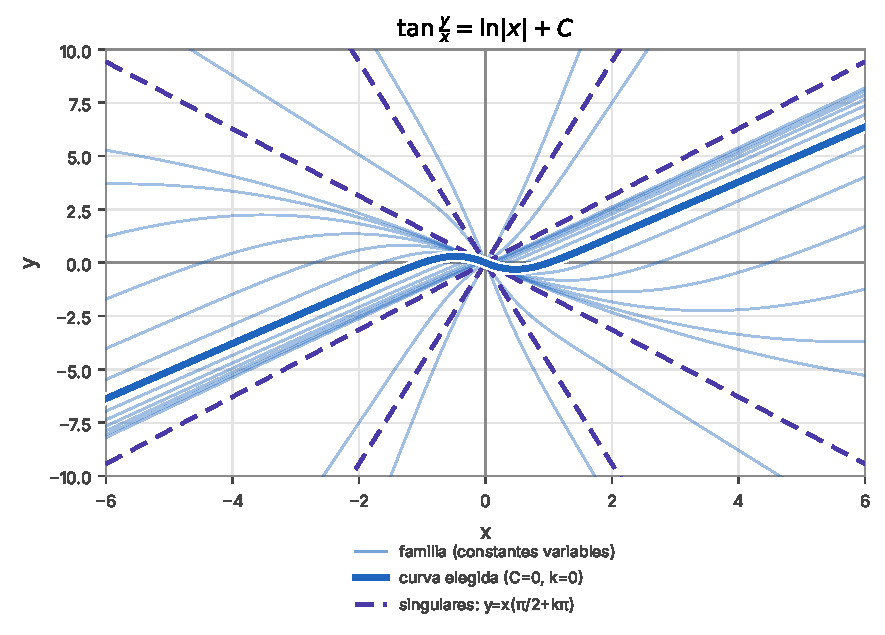
\includegraphics[width=0.8\linewidth]{h1-15.pdf}
\end{center}

\noindent\textbf{16. Integrad la EDO: $\bm{xy' = y(\ln y - \ln x)}$} \\
$z = \dfrac{y}{x} \implies y = zx \implies y' = z'x+z$; la ecuación se escribe $y' = z\ln(z)$.
\begin{align*}
z'x + z &= z\ln(z) \implies z'x = z(\ln(z)-1) \implies \frac{dz}{z(\ln(z)-1)} = \frac{dx}{x}
\end{align*}
\textit{El dominio exige $y>0$, es decir $z>0$. Al dividir por $\ln(z)-1$ se excluye $z=e$; en ese punto $z'x=e(1-1)=0$, consistente con $z$ constante, luego $y=ex$ es también solución.}

$u = \ln(z)-1 \implies du = \dfrac{dz}{z}$.
\begin{align*}
\int \frac{du}{u} &= \int \frac{dx}{x} \\
\ln|u| &= \ln|x| + C \implies \ln(z)-1 = Kx \implies \ln(y/x) = 1 + Kx
\end{align*}
$K=0$ da $y=xe^1=ex$, recuperando el caso anterior.
\[
\boxed{y = x\, e^{1+Kx}}
\]



\begin{center}
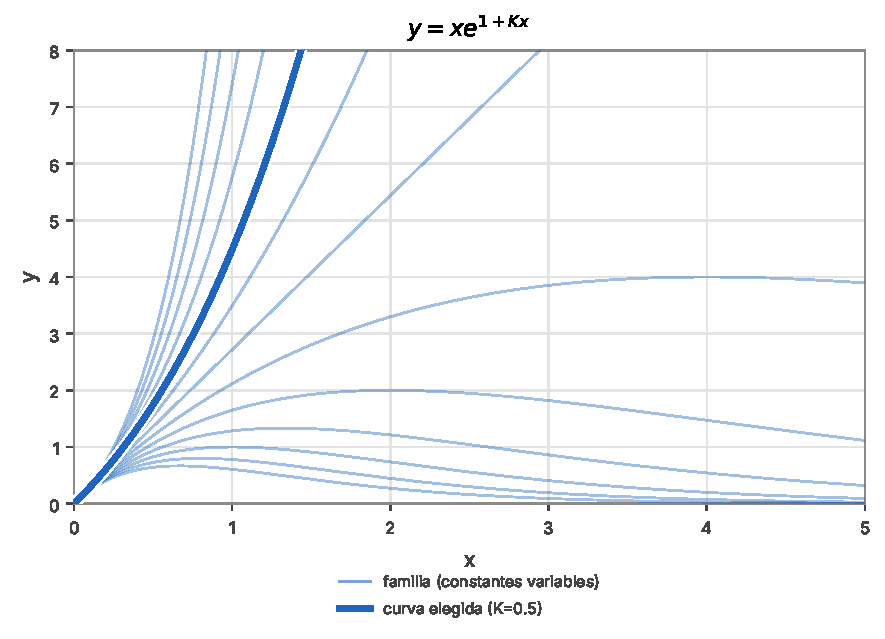
\includegraphics[width=0.8\linewidth]{h1-16.pdf}
\end{center}

\noindent\textbf{17. Integrad la EDO: $\bm{2x^2y' = x^2+y^2}$} \\
$z = \dfrac{y}{x} \implies y = zx \implies y' = z'x+z$.
\begin{align*}
z'x + z &= \frac{1+z^2}{2} \implies z'x = \frac{(z-1)^2}{2} \implies \frac{2\,dz}{(z-1)^2} = \frac{dx}{x}
\end{align*}
\textit{Al dividir por $(z-1)^2$ se excluye $z=1$; en ese punto $z'x=0$, consistente con $z$ constante. Así, $y=x$ es también solución, pero \emph{no} está contenida en la familia general (correspondería a $C\to\pm\infty$ en la expresión final).}
\begin{align*}
\int \frac{2\,dz}{(z-1)^2} &= \int \frac{dx}{x} \\
-\frac{2}{z-1} &= \ln|x| + C
\end{align*}
\[
\boxed{\frac{2x}{x-y} = \ln|x| + C}
\]



\begin{center}
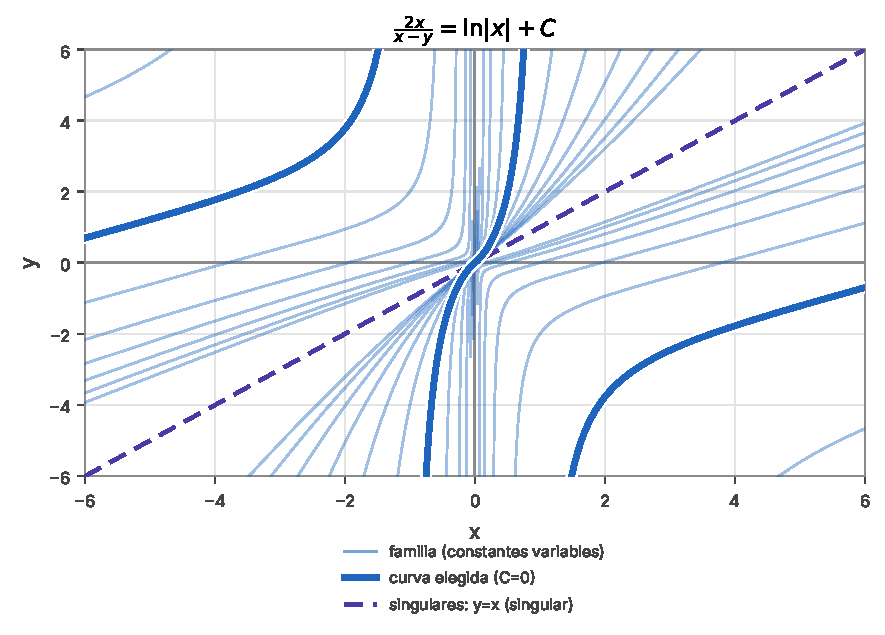
\includegraphics[width=0.8\linewidth]{h1-17.pdf}
\end{center}

\noindent\textbf{18. Integrad la EDO: $\bm{(4x-3y)dx + (2y-3x)dy = 0}$} \\
$M=4x-3y$, $N=2y-3x$. $\dfrac{\partial M}{\partial y} = -3 = \dfrac{\partial N}{\partial x}$. Buscamos la función $f(x,y)$:
\begin{align*}
f(x,y) &= \int (4x-3y)\, dx = 2x^2 - 3xy + g(y) \\
\frac{\partial f}{\partial y} &= -3x + g'(y) = 2y - 3x \implies g'(y) = 2y \implies g(y) = y^2 +K
\end{align*}

\[
\boxed{2x^2 - 3xy + y^2 = C}
\]



\begin{center}
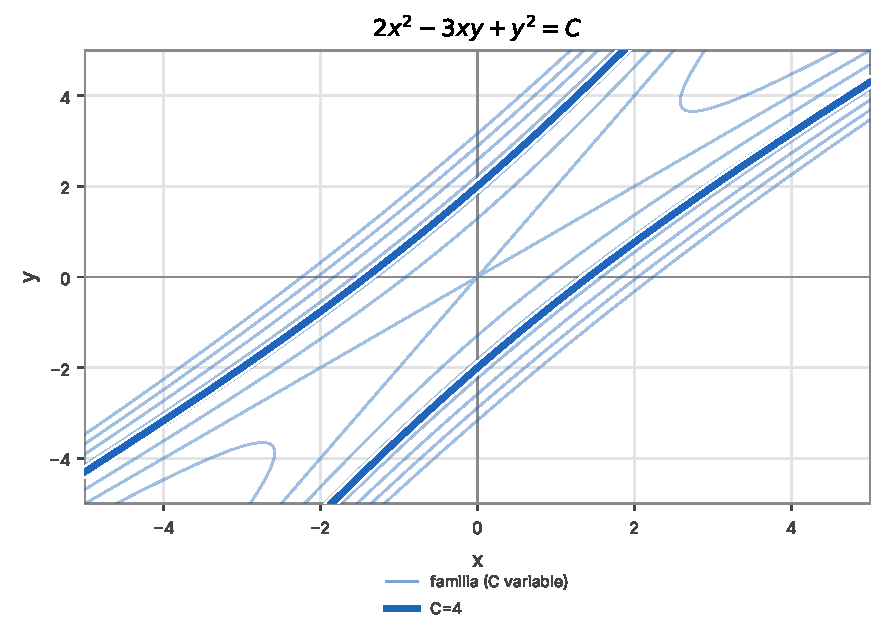
\includegraphics[width=0.8\linewidth]{h1-18.pdf}
\end{center}

\noindent\textbf{19. Integrad la EDO: $\bm{x+y-2 + (1-x)y' = 0}$} \\
Escribimos la ecuación en forma $(x+y-2)dx + (1-x)dy = 0$\\
$x=u+h$, $y=v+k$, y elegimos $h,k$ de modo que se anulen los términos independientes:
\[
\begin{cases} a_1 h + b_1 k + c_1 = 0 \\ a_2 h + b_2 k + c_2 = 0 \end{cases}
\implies
\begin{cases} h + k - 2 = 0 \\ -h + 1 = 0 \end{cases}
\]
Determinante del sistema:
\[
D = \begin{vmatrix} a_1 & b_1 \\ a_2 & b_2 \end{vmatrix} = \begin{vmatrix} 1 & 1 \\ -1 & 0 \end{vmatrix} = 1
\]
Como $D\neq 0$, el sistema tiene solución única. $h=k=1$.

\[
\frac{dv}{du} = \frac{u+v}{u} = 1+\frac{v}{u}
\]
$z = \dfrac{v}{u} \implies v=zu \implies \dfrac{dv}{du}=z'u+z$.
\begin{align*}
z'u+z &= 1+z \implies z'u = 1 \implies \int dz = \int \frac{du}{u} \implies z = \ln|u| + C
\end{align*}
\[
\frac{y-1}{x-1} = \ln|x-1| + C
\]
\[
\boxed{y = 1 + (x-1)\big(\ln|x-1| + C\big)}
\]



\begin{center}
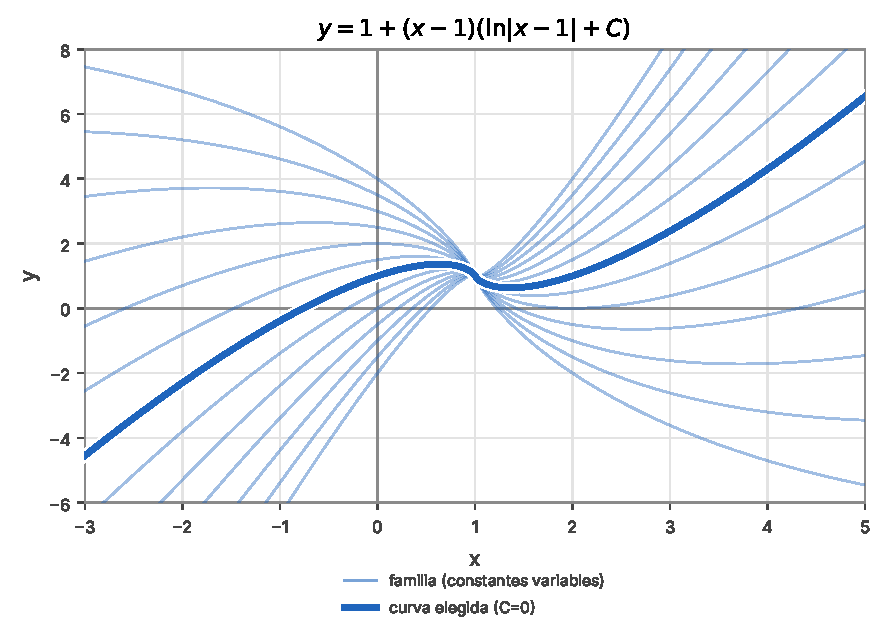
\includegraphics[width=0.8\linewidth]{h1-19.pdf}
\end{center}

\noindent\textbf{20. Integrad la EDO: $\bm{(3y-7x+7)dx - (3x-7y-3)dy = 0}$} \\
Analogamente al 19. :
\[
\begin{cases} a_1 h + b_1 k + c_1 = 0 \\ a_2 h + b_2 k + c_2 = 0 \end{cases}
\implies
\begin{cases} -7h + 3k = -7 \\ -3h + 7k = -3 \end{cases}
\]
Determinante del sistema:
\[
D = \begin{vmatrix} a_1 & b_1 \\ a_2 & b_2 \end{vmatrix} = \begin{vmatrix} -7 & 3 \\ -3 & 7 \end{vmatrix} = -49+9 = -40
\]

\[
-49h+21k=-49, \qquad -9h+21k=-9 \implies -40h=-40 \implies h=1
\]
\[
h=1, \qquad k=0
\]

\[
\frac{dv}{du} = \frac{-7u+3v}{3u-7v} = \frac{-7+3(v/u)}{3-7(v/u)}
\]
$z = \dfrac{v}{u} \implies v=zu \implies \dfrac{dv}{du}=z'u+z$.
\begin{align*}
z'u+z &= \frac{3z-7}{3-7z} \implies z'u = \frac{3z-7-z(3-7z)}{3-7z} = \frac{7(z^2-1)}{3-7z}
\end{align*}
\textit{Al dividir por $u=x-1$ se excluye $x=1$, correspondiente al punto singular $(x,y)=(1,0)$ (el centro del sistema). Además, la división por $(3-7z)$ excluye $z=3/7$ (allí las curvas tienen tangente vertical, no es una solución). Por otro lado, cuando $z^2-1=0$ (es decir $z=\pm1$) se tiene $z'u=0$, consistente con $z$ constante:}
\begin{itemize}
\item $z=1 \Rightarrow v=u \Rightarrow y=x-1$. Comprobación: con $dy=dx$, $(3y-7x+7)-( 3x-7y-3)=(-4x+4)-(-4x+4)=0$ \checkmark.
\item $z=-1 \Rightarrow v=-u \Rightarrow y=1-x$. Comprobación: con $dy=-dx$, $(3y-7x+7)+(3x-7y-3)=-4y-4x+4=0$ \checkmark.
\end{itemize}
Ambas rectas son, por tanto, soluciones singulares.

\[
\frac{3-7z}{7(z^2-1)}dz = (\dfrac{-2/7}{z-1} - \dfrac{5/7}{z+1} )dz = \frac{du}{u}
\]

\begin{align*}
\int \left(\frac{-2/7}{z-1} - \frac{5/7}{z+1}\right)dz &= \int \frac{du}{u} \\
-\frac{2}{7}\ln|z-1| - \frac{5}{7}\ln|z+1| &= \ln|u| + K_1 \\
7\ln|u| + 2\ln|z-1| + 5\ln|z+1| &= C
\end{align*}

\[
u^7\left(\frac{v}{u}-1\right)^2\left(\frac{v}{u}+1\right)^5 = C_2 \implies (v-u)^2(v+u)^5 = C_2
\]
\[
\boxed{(y-x+1)^2(y+x-1)^5 = C_3}
\]


\begin{center}
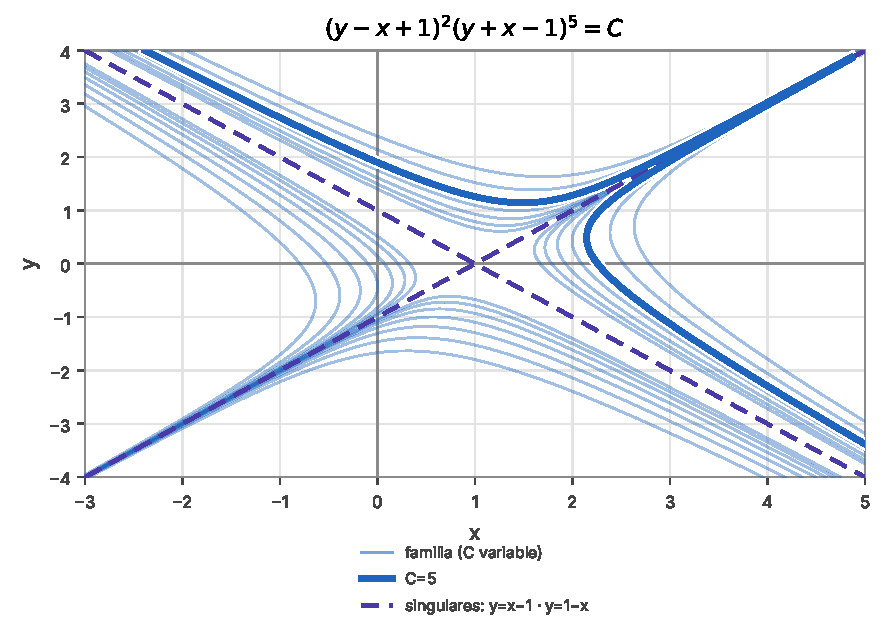
\includegraphics[width=0.8\linewidth]{h1-20.pdf}
\end{center}

\separador

\end{document}
